\documentclass[10pt,conference,compsocconf]{IEEEtran}

\usepackage{hyperref}
\usepackage{graphicx}	% For figure environment


\begin{document}
\title{Recommender System}

\author{
   Asmae Tounsi, Lukas Moser, Deepak Karkala \\
  \textit{Ecole Polytechnique Federale de Lausanne, Switzerland}
}

\maketitle

\begin{abstract}
  
\end{abstract}

\section{Introduction}



\section{Methodology}
\label{sec:tips-writing}

\subsection{Brief description of data}


\subsection{Baseline methods}
\subsubsection{Global Mean}
\subsubsection{User Mean}
\subsubsection{Item Mean}

\subsection{Pre-processing}
\subsubsection{Pre processing method 1}
\subsubsection{Pre processing method 2}


\subsection{Models and Methods}
\subsubsection{Matrix factorisation}
Given the items $\mathbf{d = 1,2...D}$ and the users $\mathbf{n = 1,2...N}$, let $\mathbf{X}$ be the $\mathbf{DxN}$ data matrix containing all the rating entries.

Matrix factorization models map both users and items to a joint latent factor space of dimensionality $K$, such that user-item interactions are modeled as inner products in that space. The aim is to determine the two matrices $\mathbf{W}$, $\mathbf{Z}$ such that the data matrix $\mathbf{X}$ is approximated by 

\begin{equation}
X \approx W Z^{T}
\end{equation}  

where  $\mathbf{W}$ and $\mathbf{Z}$ are matrices of dimensions $\mathbf{DxK}$ and $\mathbf{NxK}$ respectively and 
$\mathbf{K}$ $<<$ $\mathbf{D, N}$. Each row of $\mathbf{W}$ and $\mathbf{Z}$ is the feature representation of a movie and a user respectively.

In general, the matrix $\mathbf{X}$ is very sparse. Let $\Omega$ be the indices of the observed ratings of the input matrix $\mathbf{X}$. The objective is to determine the matrices $\mathbf{W}$ and $\mathbf{Z}$ such that the following cost function is minimised.
\begin{equation}
min_{W,Z} L(W, Z) = \frac{1}{2}  \sum_{(d,n \in \Omega)} [x_{dn} - (WZ^{T}_{dn})]^2
\end{equation}

Further in order to avoid over-fitting, we can use regularisation and penalise arbitrarily large entries in $\mathbf{W}$ and $\mathbf{Z}$. In this case, we will minimise the following cost function,

\begin{equation}
\frac{1}{2}  \sum_{(d,n \in \Omega)} [x_{dn} - (WZ^{T}_{dn})]^2 + \frac{\lambda_{w}}{2} \parallel W \parallel ^{2}_{Frob} + \frac{\lambda_{z}}{2} \parallel Z \parallel ^{2}_{Frob} 
\end{equation}
where $\lambda_{w}$, $\lambda_{z}$ $>$ $\mathbf{0}$ are scalars.

The above minimisation can be done using multiple methods. In this work, we use Stochastic Gradient Descent, Alternating least squares and the Coordinate descent methods to determine the matrices $\mathbf{W}$ and $\mathbf{Z}$.


\begin{itemize}

\item{Stochastic Gradient Descent}
In this method, for each rating in training set, we predict $\mathbf{x_{d,n}}$ and compute the prediction error as 
\begin{equation}
e_{dn} = x_{dn} - (WZ^{T})_{dn}
\end{equation}
The updates can then be computed as 
\begin{equation}

\end{equation}

\item{Alternating Least Squares}
\item{Coordinate Descent}


\end{itemize}

\subsection{Results}
\subsubsection{Baseline performance}
\subsubsection{Matrix factorisation with SGD}
(Plot cross validation results)
\begin{itemize}

\item Number of features: K
\begin{figure}[h!]
  \centering
  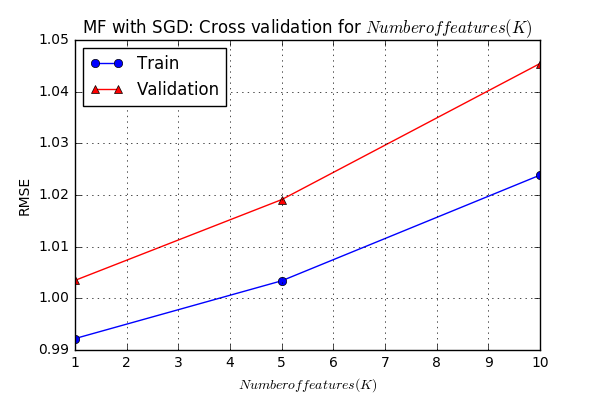
\includegraphics[width=\columnwidth]{figures/sgd_cv_numFeatures}
  \caption{Cross validation: Number of features in Matrix factorisation with SGD.}
  \vspace{-3mm}
  \label{fig:sgd_cv_numFeatures}
\end{figure}

\item Regularisation parameter: $\lambda_{user}$
\begin{figure}[h!]
  \centering
  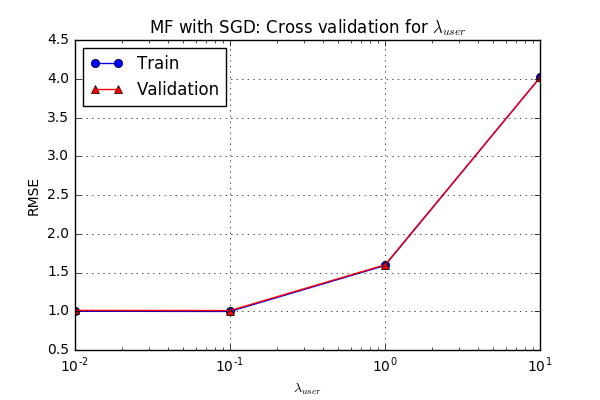
\includegraphics[width=\columnwidth]{figures/sgd_cv_lambdaUser}
  \caption{Cross validation: $\lambda_{user}$ in Matrix factorisation with SGD.}
  \vspace{-3mm}
  \label{fig:sgd_cv_lambdaUser}
\end{figure}

\item Regularisation parameter: $\lambda_{item}$
\begin{figure}[h!]
  \centering
  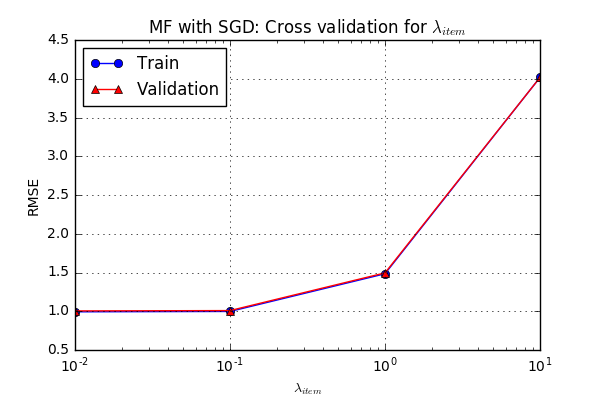
\includegraphics[width=\columnwidth]{figures/sgd_cv_lambdaItem}
  \caption{Cross validation: $\lambda_{item}$ in Matrix factorisation with SGD.}
  \vspace{-3mm}
  \label{fig:sgd_cv_lambdaItem}
\end{figure}


\item Learning rate $\gamma$
\end{itemize}
\subsubsection{Matrix factorisation with ALS}
(Plot cross validation results)
\begin{itemize}
\item Number of features: K
\item Regularisation parameter: $\lambda_{user}$
\item Regularisation parameter: $\lambda_{item}$
\end{itemize}
\subsubsection{Results with other method}
\subsubsection{Compare results for SGD, ALS, other method}


\section{Discussion}

\section{Summary}

\bibliographystyle{IEEEtran}

\end{document}
